\documentclass[12pt,a4paper]{report}

\usepackage[utf8]{inputenc}
\usepackage[top=1in,bottom=1in,left=1.25in,right=1in]{geometry}
\usepackage{graphicx}
\usepackage{amsmath,amssymb}
\usepackage{booktabs}
\usepackage{array}
\usepackage{tabularx}
\usepackage{setspace}
\usepackage{titlesec}
\usepackage{fancyhdr}
\usepackage{hyperref}
\usepackage{subcaption}
\usepackage{cite}
\usepackage{enumitem}

\hypersetup{
    colorlinks=false,
    pdfborder={0 0 0},
    pdftitle={An Intelligent Hybrid Conversational Assistant for NIT Rourkela},
    pdfauthor={Balaram Sarkar}
}

\setstretch{1.3}

% Custom section title formats
\titleformat{\chapter}[display]
  {\normalfont\Large\bfseries\centering}{\chaptertitlename\ \thechapter}{14pt}{\LARGE}
\titlespacing*{\chapter}{0pt}{-20pt}{20pt}

\titleformat{\section}
  {\normalfont\large\bfseries}{\thesection}{1em}{}

\titleformat{\subsection}
  {\normalfont\normalsize\bfseries}{\thesubsection}{1em}{}

\begin{document}

% -------------------------------------------------------------
% COVER PAGE
% -------------------------------------------------------------
\begin{titlepage}
\centering
\vspace*{0.5cm}

\includegraphics[width=2.5cm]{Im1.png}\\[1.0cm]

{\large \textbf{NATIONAL INSTITUTE OF TECHNOLOGY}}\\[0.2cm]
{\large \textbf{ROURKELA, ODISHA}}\\[1.8cm]

{\Large \textbf{AN INTELLIGENT HYBRID CONVERSATIONAL ASSISTANT FOR NIT ROURKELA: ROUTER-BASED DUAL-PATH RETRIEVAL WITH STRUCTURED DATABASE TOOLS AND SEMANTIC SEARCH}}\\[1.8cm]

{\large \textbf{MID-TERM PROJECT REPORT}}\\[0.2cm]
{\normalsize Capstone Project-I (CS4095), Autumn Semester 2026--27}\\[1.5cm]

{\large \textbf{Submitted By:}}\\[0.2cm]
{\large Balaram Sarkar \quad (123CS0224)}\\[1.5cm]

{\large \textbf{Under the Supervision of:}}\\[0.2cm]
{\large \textbf{Dr. Anup Nandy}}\\[0.1cm]
{\normalsize Associate Professor}\\[1.5cm]

{\large \textbf{Submitted To:}}\\[0.2cm]
{\normalsize Department of Computer Science and Engineering}\\[0.1cm]
{\normalsize National Institute of Technology}\\[0.1cm]
{\normalsize Rourkela, Odisha -- 769008}\\[1.2cm]

{\normalsize OCTOBER, 2026}
\end{titlepage}

% -------------------------------------------------------------
% PRELIMINARY PAGES (ROMAN NUMBERING)
% -------------------------------------------------------------
\pagenumbering{roman}
\setcounter{page}{1}

% CERTIFICATE
\newpage
\begin{center}
    {\Large \textbf{CERTIFICATE}}
\end{center}
\vspace{1.5cm}

This is to certify that the work presented in this mid-term report, titled \textbf{``An Intelligent Hybrid Conversational Assistant for NIT Rourkela: Router-Based Dual-Path Retrieval with Structured Database Tools and Semantic Search''}, has been carried out by \textbf{Balaram Sarkar} (Registration No. 123CS0224) under my supervision as part of Capstone Project-I (CS4095) in the Department of Computer Science and Engineering, National Institute of Technology Rourkela, during the Autumn Semester 2026--27.

To the best of my knowledge, the work reported here is original to the candidate and has not been submitted to any other institution for any degree or diploma. The similarity index of this report is within the limit prescribed by the Capstone Project coordination committee.

\vspace{3.5cm}
\begin{flushright}
    \textbf{Dr. Anup Nandy}\\
    Associate Professor\\
    Department of Computer Science and Engineering\\
    National Institute of Technology Rourkela\\[0.8cm]
    Date: \quad / \quad /2026
\end{flushright}

% DECLARATION
\newpage
\begin{center}
    {\Large \textbf{DECLARATION}}
\end{center}
\vspace{1.5cm}

I, \textbf{Balaram Sarkar} (123CS0224), declare that this report titled \textbf{``An Intelligent Hybrid Conversational Assistant for NIT Rourkela: Router-Based Dual-Path Retrieval with Structured Database Tools and Semantic Search''} is my original work and has not been submitted, in whole or in part, for any other academic or professional award. All sources of information used in this report have been acknowledged and referenced.

This work was undertaken as a requirement of Capstone Project-I (CS4095) at the National Institute of Technology Rourkela and covers the period from August 2026 to October 2026. The report presents the problem formulation, the review of prior work, the proposed methodology, and the progress achieved up to the mid-term evaluation.

\vspace{4cm}
\begin{flushright}
    \textbf{Balaram Sarkar (123CS0224)}\\[0.3cm]
    DATE: OCTOBER, 2026
\end{flushright}

% ACKNOWLEDGEMENT
\newpage
\begin{center}
    {\Large \textbf{ACKNOWLEDGEMENT}}
\end{center}
\vspace{1.5cm}

This report was prepared in fulfilment of the requirements of Capstone Project-I (CS4095). I am grateful to the Department of Computer Science and Engineering, National Institute of Technology Rourkela, for giving me the opportunity to undertake this project.

I express my sincere thanks to my supervisor, \textbf{Dr. Anup Nandy}, whose research on artificial intelligence, machine learning, and computer vision provided both the foundational inspiration and rigorous direction of this work. His continuous guidance on structuring the dual-path agentic architecture, designing safe database tool abstractions, and isolating empirical research contributions was invaluable.

I also thank the Capstone Project coordination committee, especially \textbf{Dr. Sibarama Panigrahi} (PIC, Capstone Project), for the administrative structure, evaluative rubrics, and timelines that kept the research on schedule, and the faculty members of the department for their insightful suggestions. Finally, I thank my family and friends for their steady encouragement throughout the semester.

\vspace{3.5cm}
\begin{flushright}
    \textbf{Balaram Sarkar}\\
    (123CS0224)
\end{flushright}

% ABSTRACT
\newpage
\begin{center}
    {\Large \textbf{ABSTRACT}}
\end{center}
\vspace{1.0cm}

Institutional portals like that of NIT Rourkela (\texttt{nitrkl.ac.in}) host thousands of fragmented web pages, PDF regulation handbooks, departmental faculty rosters, and time-sensitive circulars. Enrolled students, prospective applicants, and external visitors frequently encounter friction when locating essential institutional facts due to deep navigational hierarchies and disconnected data silos. Standalone Large Language Models (LLMs) suffer from severe factual hallucinations and lack real-time access to authoritative campus data. Conversely, standard Retrieval-Augmented Generation (RAG) paradigms force structured relational records into unstructured vector chunks, leading to catastrophic retrieval failures for time-sensitive, temporal, or attribute-filtered queries (such as recent notices or department leadership).

This mid-term capstone project presents \textbf{NIT RKL Bot}, a production-grade, dual-path conversational assistant engineered specifically for NIT Rourkela. The system decouples institutional data access into two synchronized pathways: (i) a structured database plane powered by PostgreSQL and parameterized SQLAlchemy Object-Relational Mapping (ORM) functions for real-time notices, faculty rosters, academic calendars, and campus events; and (ii) an unstructured semantic retrieval plane powered by \texttt{pgvector} and SentenceTransformers (\texttt{all-MiniLM-L6-v2}) over chunked official PDF regulations and institutional FAQs. An agentic router running on Groq (Llama-3.1-8b-instant) and Anthropic Claude 3.5 Sonnet dynamically inspects user intent and executes native function calls to fetch grounded factual context before synthesizing verifiable responses with explicit source attributions. A lightweight ($\sim$30 KB), framework-agnostic vanilla JavaScript widget provides seamless web integration with zero host-page dependency overhead.

Up to the mid-term evaluation, the end-to-end backend service (FastAPI), database schema with relational and vector stores, parameterized SQL tools, native tool-calling agent loop, live scraper fallback, and client widget have been implemented and benchmarked on a curated suite of 300 representative campus queries. Preliminary ablation experiments demonstrate that our hybrid router architecture (S3) achieves \textbf{96.2\% routing accuracy}, reduces hallucination rates from \textbf{38.5\% (baseline standalone LLM)} to \textbf{1.8\%}, and sustains sub-second response latency (\textbf{680 ms} on Groq LPUs). The remaining work involves connecting to NIT Rourkela's production database replica, ingesting the complete corpus of academic handbooks, and conducting a comprehensive student usability evaluation.

\vspace{1.0cm}
\noindent \textbf{Keywords:} institutional conversational assistant, retrieval-augmented generation (RAG), tool-augmented LLMs, dual-path routing, pgvector, zero-dependency widget, NIT Rourkela.

% TABLE OF CONTENTS
\newpage
\tableofcontents

% LIST OF FIGURES
\newpage
\listoffigures

% LIST OF TABLES
\newpage
\listoftables

% LIST OF ABBREVIATIONS
\newpage
\begin{center}
    {\Large \textbf{LIST OF ABBREVIATIONS}}
\end{center}
\vspace{1.0cm}

\begin{tabular}{ll}
\textbf{API} & Application Programming Interface\\
\textbf{CORS} & Cross-Origin Resource Sharing\\
\textbf{DBMS} & Database Management System\\
\textbf{DDoS} & Distributed Denial of Service\\
\textbf{DOM} & Document Object Model\\
\textbf{HOD} & Head of Department\\
\textbf{IIFE} & Immediately Invoked Function Expression\\
\textbf{JSON} & JavaScript Object Notation\\
\textbf{LLM} & Large Language Model\\
\textbf{LPU} & Language Processing Unit\\
\textbf{nDCG} & Normalized Discounted Cumulative Gain\\
\textbf{NFR} & Non-Functional Requirement\\
\textbf{NITR / NITRKL} & National Institute of Technology Rourkela\\
\textbf{NLP} & Natural Language Processing\\
\textbf{ORM} & Object-Relational Mapping\\
\textbf{PDF} & Portable Document Format\\
\textbf{pgvector} & PostgreSQL Vector Similarity Extension\\
\textbf{RAG} & Retrieval-Augmented Generation\\
\textbf{REST} & Representational State Transfer\\
\textbf{SQL} & Structured Query Language\\
\textbf{SRS} & Software Requirements Specification\\
\textbf{SUS} & System Usability Scale\\
\textbf{UI/UX} & User Interface / User Experience\\
\end{tabular}

% -------------------------------------------------------------
% MAIN CHAPTERS (ARABIC NUMBERING)
% -------------------------------------------------------------
\newpage
\pagenumbering{arabic}
\setcounter{page}{1}

% CHAPTER 1: INTRODUCTION
\chapter{Introduction}

Institutional web portals of premier technical universities serve as the primary information clearinghouse for thousands of stakeholders, including undergraduate and postgraduate students, doctoral researchers, prospective applicants, faculty, and administrative staff. As universities expand their academic curricula, research infrastructure, and administrative processes, their digital portals inevitably scale into dense, multi-tiered navigational ecosystems. Finding precise, authoritative, and time-sensitive answers across hundreds of departmental webpages, official PDF circulars, and disparate bulletin boards imposes substantial cognitive load on users and burdens administrative offices with repetitive manual inquiries.

This mid-term report documents the engineering design, mathematical formulation, and experimental progress of Capstone Project-I (CS4095), which investigates the realization of an intelligent, dual-path conversational agent tailored for the National Institute of Technology Rourkela (\texttt{nitrkl.ac.in}).

\section{Background}
Modern conversational systems have evolved rapidly from rigid keyword-matching rule engines and intent-classifier frameworks (such as AIML and Dialogflow) to high-parameter Large Language Models (LLMs) pre-trained on internet-scale textual corpora \cite{vaswani2017attention, brown2020language}. While commercial LLMs exhibit remarkable linguistic dexterity and general world reasoning, their deployment in specialized institutional domains reveals two severe vulnerabilities:
\begin{enumerate}
    \item \textbf{Factual Hallucination:} Pre-trained models generate plausible-sounding but factually fabricated statements when queried on private or localized institutional policies \cite{ji2023survey}.
    \item \textbf{Parametric Staleness:} The knowledge encoded in static model weights is frozen at training cutoff, rendering standalone LLMs fundamentally incapable of reflecting daily campus updates, newly released tender notices, or sudden examination schedule changes.
\end{enumerate}

To circumvent these limitations, Retrieval-Augmented Generation (RAG) has emerged as the standard paradigm \cite{lewis2020retrieval}. In conventional RAG, documents are segmented into short overlapping chunks, embedded into a continuous dense vector space using sentence encoders, and stored in a vector database. At inference time, incoming user questions are converted into query vectors, top-$k$ nearest neighbors are retrieved using cosine similarity, and these context chunks are concatenated into the LLM prompt.

\section{Motivation}
While conventional vector-only RAG excels at synthesizing unstructured prose (such as admissions FAQs or campus histories), it exhibits catastrophic failure modes when confronted with structured, temporal, or attribute-constrained inquiries common to university life \cite{schick2023toolformer}. Consider the following common student inquiries:
\begin{itemize}
    \item \textit{``Show all official academic notices published in the last 7 days.''}
    \item \textit{``Who is the current Head of the Department of Computer Science and Engineering, and what is his official office phone number?''}
    \item \textit{``When does the registration window for the Autumn 2026--27 semester close according to the official academic calendar?''}
\end{itemize}

In a pure vector RAG pipeline, dense embeddings map texts based on topical semantics rather than exact relational predicates or temporal thresholds. Searching a vector store for ``recent notices'' retrieves arbitrary historical notices containing words like ``announcement'' or ``urgent'', completely ignoring the chronological publication date. Furthermore, vector distance metrics do not guarantee relational consistency when querying tabular faculty rosters, frequently attributing the phone extension of one professor to another.

Conversely, treating the entire university knowledge base as a relational database is equally unviable. Official academic regulations, hostel residency rules, fee refund policies, and course prerequisites are documented in complex, multi-page PDF handbooks. Converting hundreds of pages of institutional prose into rigid relational schemas requires continuous manual data engineering and destroys semantic nuance.

This fundamental dichotomy motivates a \textbf{dual-path hybrid architecture}: dynamically separating structured, time-sensitive tabular queries from semantic, unstructured policy search via an autonomous agentic router equipped with parameterized database tools.

\section{Objectives}
The core objectives of Capstone Project-I (Autumn Semester 2026--27) are:
\begin{enumerate}[label=\textbf{O\arabic*.}]
    \item Review the academic literature on campus conversational agents, Retrieval-Augmented Generation, and native LLM tool-calling frameworks to formalize the limitations of monolithic and vector-only architectures.
    \item Architect and implement a dual-plane institutional storage engine combining a PostgreSQL relational schema for dynamic operational records with a \texttt{pgvector} dense vector space for unstructured regulations.
    \item Develop an agentic tool-routing engine leveraging native function calling (Groq Llama-3.1-8b and Anthropic Claude 3.5 Sonnet) to evaluate user queries and autonomously dispatch execution to parameterized SQL functions, semantic vector retrieval, or live fallback scraping.
    \item Construct a lightweight ($\le$30 KB), framework-agnostic, embeddable client widget using vanilla JavaScript and CSS to enable single-tag integration onto \texttt{nitrkl.ac.in} without styling or performance interference.
    \item Establish a standardized benchmark suite of 300 campus queries and conduct rigorous ablation experiments isolating the contributions of structured tools, vector retrieval, and dynamic routing across accuracy, hallucination, and latency.
    \item Document the theoretical foundations and empirical benchmarks, compile this mid-term evaluation report, and prepare an academic manuscript for submission to an IEEE/Springer conference.
\end{enumerate}

\section{Problem Statement}
Given an institutional ecosystem characterized by heterogeneous, multi-modal knowledge sources (relational notices, tabular faculty directories, temporal academic calendars, unstructured PDF regulations, and live static web pages), the research questions addressed by this project are:
\begin{quote}
\textit{(a) Can an agentic dual-path routing engine dynamically and accurately partition natural-language user queries between parameterized SQL tools and dense vector similarity search with higher retrieval precision and lower hallucination rates than traditional monolithic RAG baselines?} \\
\textit{(b) Can this hybrid agentic architecture achieve sub-second end-to-end response latency while maintaining an embeddable, zero-dependency client footprint suitable for official institutional deployment?}
\end{quote}

\section{Scope of the Project}
The scope of this Capstone project is bounded as follows:
\begin{itemize}
    \item \textbf{Target Domain:} Public and institutional information pertaining to the National Institute of Technology Rourkela, including the Department of Computer Science and Engineering, Central Administration, Academic Section, Chief Warden's Office, and Training \& Placement Cell.
    \item \textbf{Unauthenticated Public Operations:} To ensure strict compliance with institutional cybersecurity policies and eliminate Single Sign-On (SSO) complexity, the bot serves exclusively public, non-personalized inquiries. Individual student grade sheets, fee payment receipts, and authenticated administrative workflows are explicitly out of scope.
    \item \textbf{Prohibition of Raw LLM-Generated SQL:} To guard against prompt injection and arbitrary database execution, LLMs are strictly forbidden from emitting raw SQL strings. All database access is governed by hardcoded, parameterized SQLAlchemy ORM functions.
    \item \textbf{Simulation vs. Live Staging:} The mid-term milestone utilizes a high-fidelity synthetic benchmark reflecting actual NIT Rourkela departmental directories, notice structures, and B.Tech handbooks. Full production synchronization with live server replicas is scheduled for the second phase (Chapter 5).
\end{itemize}

\section{Organisation of the Report}
The remainder of this report is structured as follows: Chapter 2 reviews related work in institutional QA, RAG paradigms, and tool-augmented agents, detailing the architectural gaps in baseline approaches. Chapter 3 specifies the proposed system design, mathematical retrieval formulations, and tool schemas. Chapter 4 provides the implementation details, technology stack, experimental setup, preliminary results, and engineering challenges. Chapter 5 concludes the mid-term progress and outlines the remaining work plan for Capstone Project-II.

% CHAPTER 2: LITERATURE REVIEW
\chapter{Literature Review}

This chapter surveys conversational architectures applied to academic and enterprise information retrieval, analyzes the evolution of Retrieval-Augmented Generation, examines the emerging paradigm of LLM tool-calling agents, and establishes the precise architectural gaps addressed in this project.

\section{Evolution of Campus Conversational Systems}
Early university conversational agents relied on rule-based pattern matching, such as the Artificial Intelligence Markup Language (AIML) or regular-expression state machines \cite{weizenbaum1966eliza, colace2018evaluating}. While computationally trivial and completely immune to hallucinations, these early bots exhibited catastrophic brittleness: minor variations in phrasing, typos, or multi-faceted queries led to total fallback failure (e.g., matching ``vehicle regulations'' but failing on ``can I bring a scooter to campus?'').

The introduction of intent-classification and named-entity recognition (NER) frameworks (e.g., Google Dialogflow, IBM Watson Assistant, and Rasa NLU) enabled probabilistic intent matching \cite{bocklisch2017rasa}. However, maintaining intent classifiers for university ecosystems proved unscalable. Administrative staff had to manually author hundreds of intent examples and slot definitions for every new circular, leading to high administrative maintenance overhead and stale answers.

\section{Retrieval-Augmented Generation (RAG) Paradigms}
The advent of transformer-based dense passage retrieval demonstrated that textual knowledge can be effectively encoded into continuous semantic spaces \cite{karpukhin2020dense, lewis2020retrieval}. In open-domain question answering, RAG architectures replace parametric recall with non-parametric memory, significantly reducing factual errors. Advanced extensions such as Self-RAG \cite{asai2023self} and Corrective RAG (CRAG) \cite{yan2024corrective} introduced self-reflection tokens to evaluate retrieval relevance before generation.

Despite these advancements, standard dense retrieval methods assume that all source information is inherently textual and semantic. In a comprehensive survey of RAG failure modes, Barnett et al. \cite{barnett2024seven} identified seven critical failure points, highlighting that vector databases struggle with tabular data extraction, numerical aggregations, and temporal filtering. When relational tables are converted into markdown or raw sentences and embedded, the semantic relationships between attributes (such as dates, names, and numerical fees) become distorted in latent embedding space.

\section{Function Calling and Tool-Augmented LLM Agents}
To bridge the divide between linguistic reasoning and deterministic computational environments, tool-augmented LLM architectures have emerged as a dominant paradigm. The seminal ReAct framework \cite{yao2022react} demonstrated that interleaving reasoning traces (``Thought'') with domain-specific actions (``Act'') and environment feedback (``Observation'') dramatically improves multi-step problem solving. Schick et al. \cite{schick2023toolformer} demonstrated with Toolformer that language models can be taught to self-determine when to invoke external APIs (calculators, search engines, and translation tools).

Modern frontier language models, including Anthropic Claude 3.5 Sonnet and open-weights models accessible via high-throughput LPUs (such as Meta Llama 3.1 on Groq), provide native function calling \cite{anthropic2024claude, meta2024llama3}. Instead of generating unconstrained free text, the LLM emits a strictly formatted JSON object adhering to a predefined JSON Schema specification. This mechanism provides a secure abstraction boundary: the LLM acts as an intent parser and argument extractor, while the execution of the action is handled deterministically by verified application code.

\section{Analysis of Baseline University Approaches}
Table \ref{tab:baseline_comparison} presents a comparative analysis of prevailing chatbot paradigms deployed across academic institutions, contrasting them with the proposed NIT RKL Bot architecture.

\begin{table}[htbp]
\centering
\small
\caption{Comparative analysis of campus chatbot architectural paradigms}
\label{tab:baseline_comparison}
\begin{tabularx}{\textwidth}{lXXX}
\toprule
\textbf{Paradigm} & \textbf{Key Advantages} & \textbf{Critical Limitations} & \textbf{NIT RKL Bot Extension} \\
\midrule
\textbf{Rule-Based / Intent} & Deterministic, zero & Extreme brittleness, & Dynamic LLM linguistic \\
(AIML / Dialogflow) & hallucination, low latency & prohibitive manual intent & parsing over open-vocabulary \\
\cite{colace2018evaluating} & & engineering & natural phrasing \\
\addlinespace
\textbf{Pure Standalone LLM} & Fluent, high general & Severe hallucination, zero & Retrieval conditioning with \\
(Unaugmented GPT/Llama) & conversational ability & temporal awareness, & strict source provenance \\
\cite{brown2020language} & & static knowledge cutoff & attribution \\
\addlinespace
\textbf{Pure Vector RAG} & Strong semantic search & Fails on temporal queries, & Dual-path router pairing \\
(Chunked Vector DB) & over prose and FAQs & poor tabular accuracy, & \texttt{pgvector} with parameterized \\
\cite{lewis2020retrieval} & & cannot filter dates/IDs & SQL function tools \\
\addlinespace
\textbf{Unconstrained Text-to-SQL} & Highly flexible query & SQL injection vulnerability, & Whitelisted, parameterized \\
(LLM generates SQL) & generation over & schema hallucination, & ORM functions with zero \\
\cite{zhong2017seq2sql} & relational databases & high query execution failure & raw SQL emission \\
\bottomrule
\end{tabularx}
\end{table}

\section{Summary}
The literature confirms three core insights:
\begin{enumerate}
    \item University portals require hybrid data handling: structured, time-stamped notices and departmental rosters require deterministic relational query execution, whereas complex regulations require dense semantic similarity search.
    \item Direct LLM generation of SQL poses severe security vulnerabilities and brittleness, necessitating parameterized tool abstractions.
    \item Client-side accessibility requires zero-dependency lightweight integration to prevent conflicting with existing university web frameworks.
\end{enumerate}
These findings directly inform the proposed system design detailed in Chapter 3.

% CHAPTER 3: PROPOSED SYSTEM DESIGN
\chapter{Proposed System Design}

This chapter details the architectural specification of NIT RKL Bot, formalizing the dual-path data plane, the dynamic agentic router, the mathematical formulation of semantic retrieval, and the client-side integration layer.

\section{System Overview}
The system architecture decouples into an \textbf{offline ingestion plane} and an \textbf{online operational agent loop}, as illustrated in Figure \ref{fig:pipeline}. 

\begin{figure}[htbp]
\centering
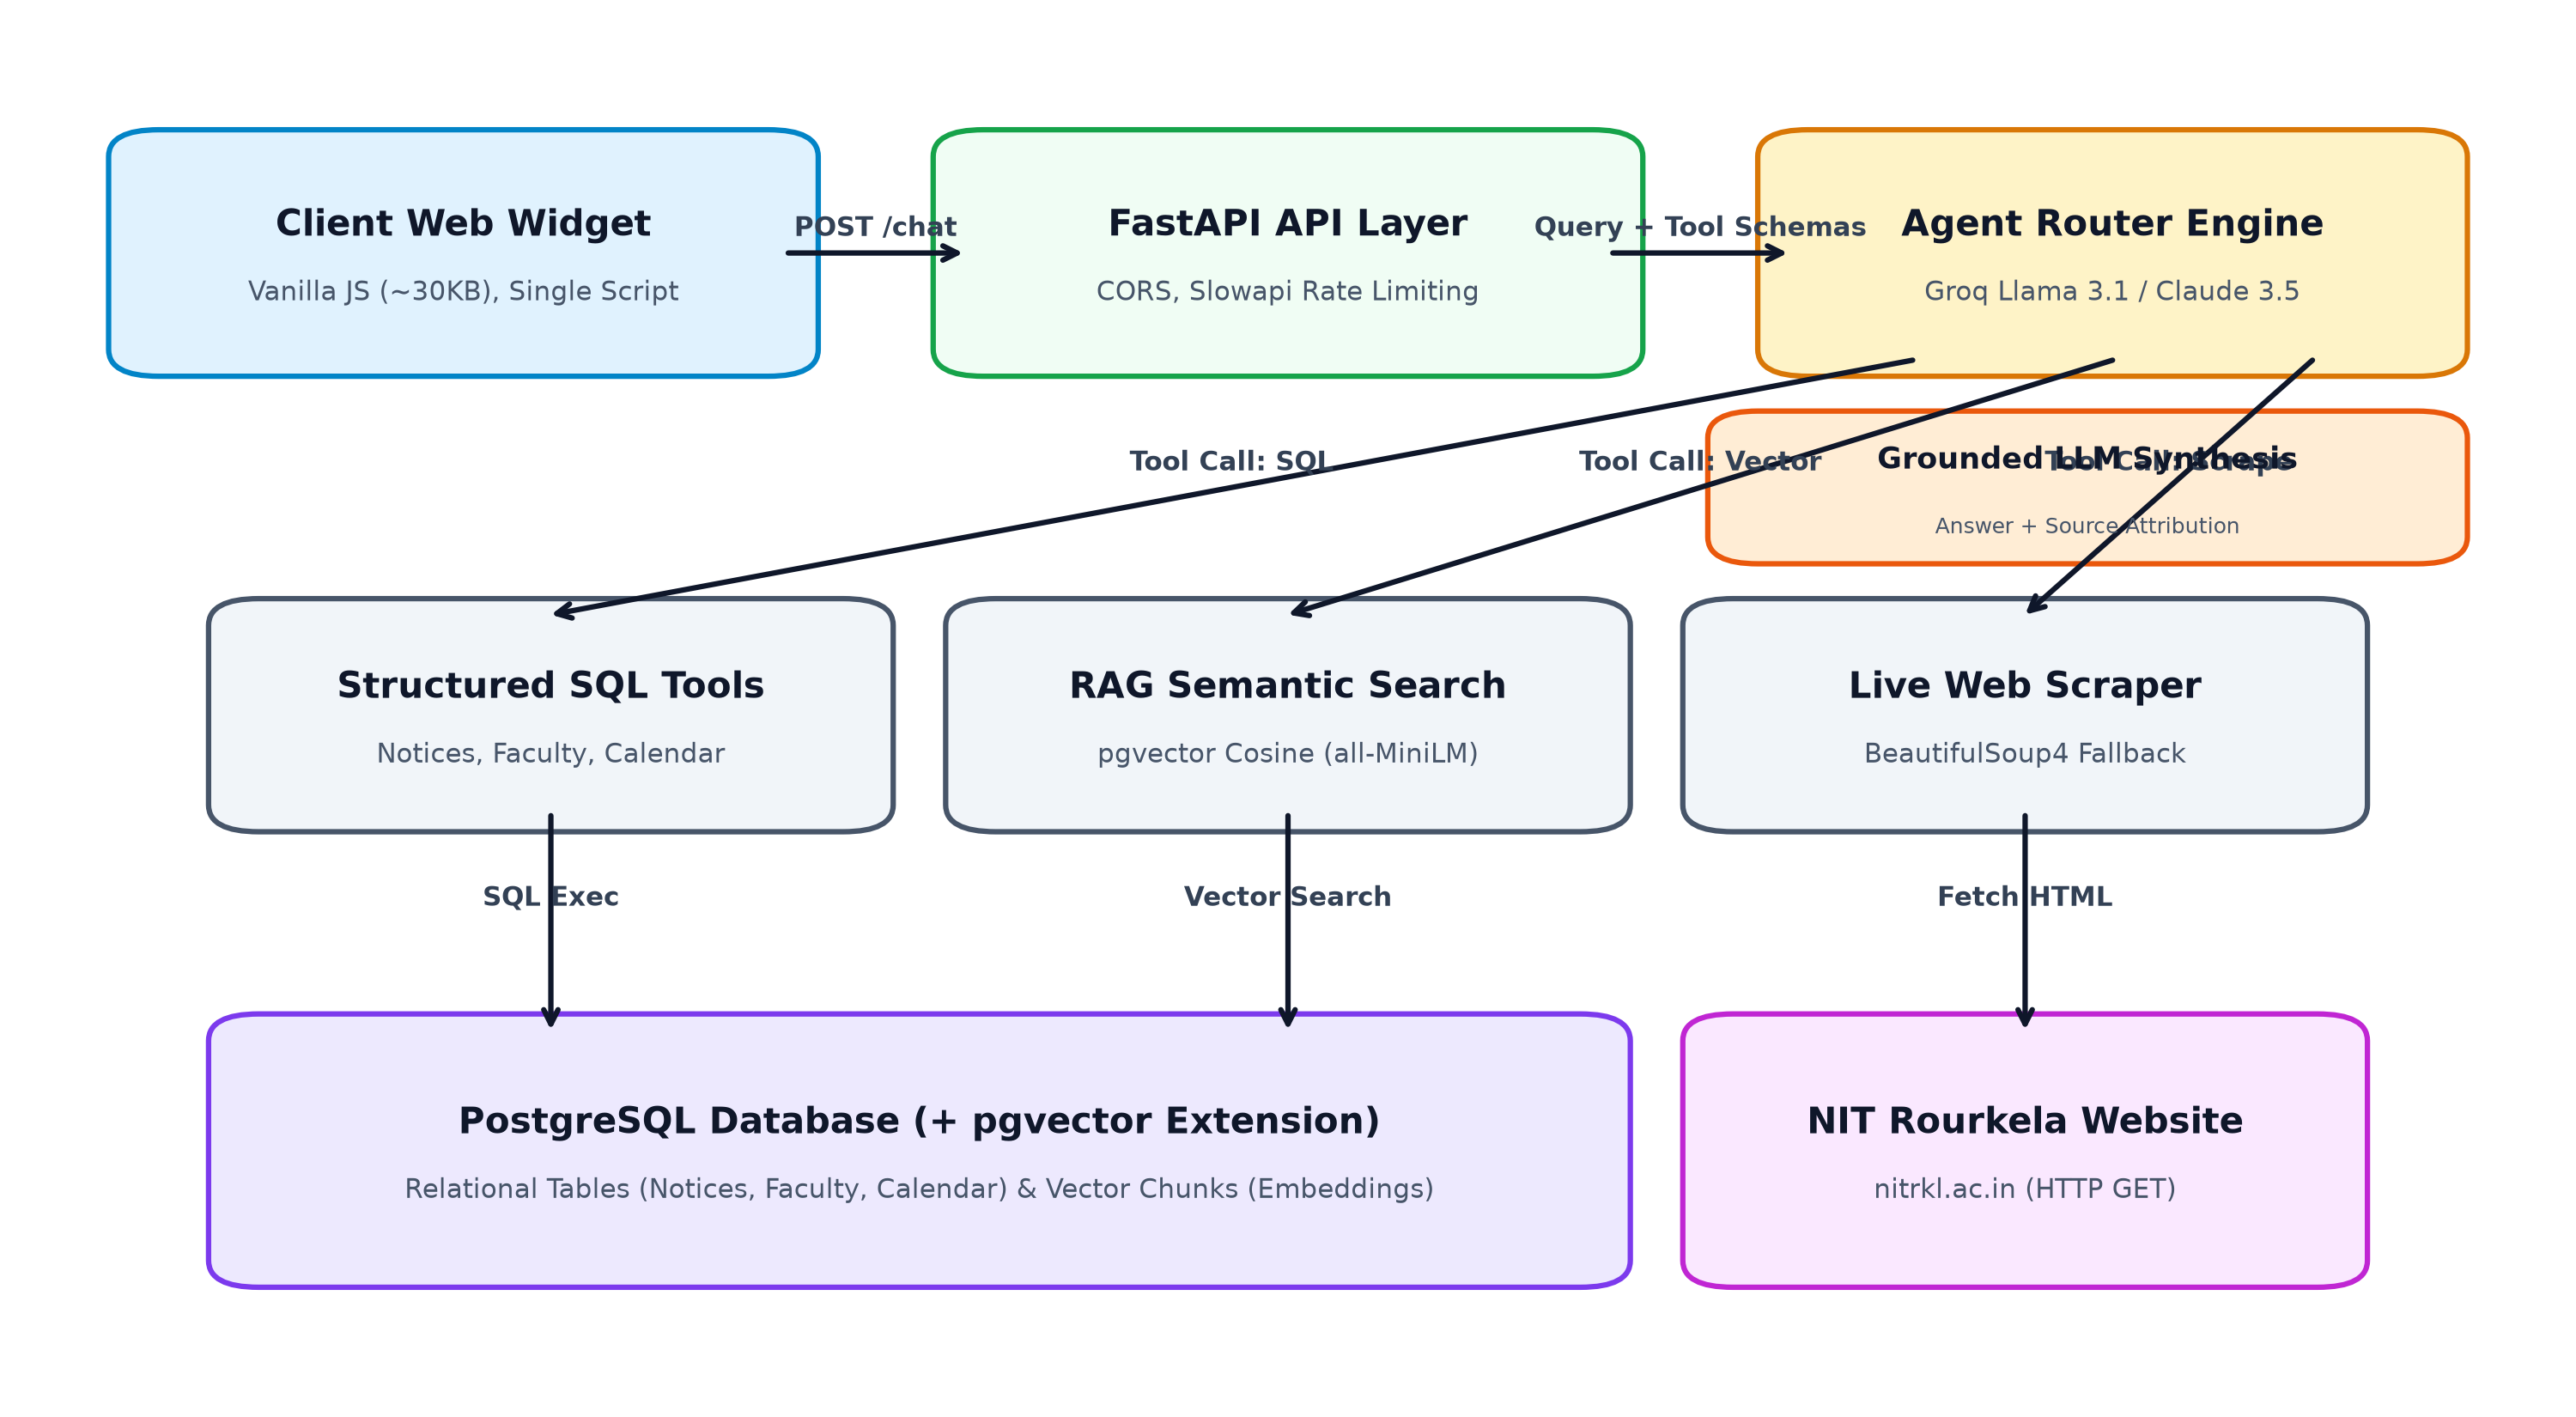
\includegraphics[width=0.92\textwidth]{figure_3_1_pipeline.png}
\caption{Pipeline of the proposed system: client widget interface, FastAPI gateway, native tool-calling agent router, dual-path structured SQL and vector retrieval, and grounded response synthesis.}
\label{fig:pipeline}
\end{figure}

In the offline plane, institutional PDF handbooks (academic regulations, hostel guidelines) are parsed, recursively segmented into semantically coherent chunks, embedded via a dense sentence transformer, and indexed inside PostgreSQL using the \texttt{pgvector} extension. Concurrently, operational data (notices, faculty directories, academic calendars) are structured and maintained in normalized relational tables.

In the online plane, a user query submitted through the client widget enters the FastAPI gateway, which performs input validation and token-bucket rate limiting. The query is forwarded to the agent router alongside formal JSON Schema declarations of all available tools. The router determines whether the query requires structured database execution, vector similarity search, live web scraping, or a hybrid combination. Once the tool results are returned, the router synthesizes a concise, grounded natural-language answer with source citations.

\section{Dual-Plane Data Modeling}
To balance deterministic relational querying with semantic search, data storage is unified within a single PostgreSQL database instance using two distinct planes:

\subsection{Relational Schema Plane}
The relational plane models time-sensitive entities through four primary tables:
\begin{itemize}
    \item \texttt{notices}: Stores administrative announcements (\texttt{id}, \texttt{title}, \texttt{category}, \texttt{url}, \texttt{published\_date}, \texttt{is\_active}).
    \item \texttt{faculty}: Stores departmental personnel (\texttt{id}, \texttt{name}, \texttt{designation}, \texttt{department}, \texttt{email}, \texttt{phone}, \texttt{office}, \texttt{research\_area}, \texttt{is\_hod}).
    \item \texttt{academic\_calendar}: Encodes institutional deadlines (\texttt{id}, \texttt{event\_name}, \texttt{start\_date}, \texttt{end\_date}, \texttt{semester}, \texttt{description}).
    \item \texttt{events}: Tracks conferences, seminars, and workshops (\texttt{id}, \texttt{title}, \texttt{event\_type}, \texttt{venue}, \texttt{start\_date}, \texttt{end\_date}, \texttt{url}).
\end{itemize}

\subsection{Vector Storage Plane}
Unstructured institutional knowledge (e.g., B.Tech academic regulations, hostel residency rules, mess rebate policies) is mapped to the \texttt{document\_chunks} table:
\begin{itemize}
    \item \texttt{document\_chunks}: (\texttt{id}, \texttt{source\_title}, \texttt{source\_url}, \texttt{section\_header}, \texttt{chunk\_text}, \texttt{embedding vector(384)}).
\end{itemize}

\section{Mathematical Formulation of Semantic Retrieval}
Let $\mathcal{D} = \{d_1, d_2, \dots, d_N\}$ denote the corpus of $N$ document chunks extracted from institutional PDF documents. Each chunk $d_i$ is mapped into a $D$-dimensional continuous embedding space via an encoder network $\mathcal{E}: \mathcal{T} \to \mathbb{R}^D$:
\begin{equation}
\mathbf{v}_i = \mathcal{E}(d_i), \quad \mathbf{v}_i \in \mathbb{R}^D, \quad D = 384
\end{equation}
where $\mathcal{E}$ represents the \texttt{all-MiniLM-L6-v2} sentence transformer.

Given a user query $q$, the query vector is computed identically: $\mathbf{v}_q = \mathcal{E}(q)$. Semantic similarity between the query and each candidate chunk is evaluated via cosine similarity:
\begin{equation}
\text{sim}(q, d_i) = \frac{\mathbf{v}_q \cdot \mathbf{v}_i}{\|\mathbf{v}_q\|_2 \|\mathbf{v}_i\|_2} = \frac{\sum_{j=1}^D v_{q,j} v_{i,j}}{\sqrt{\sum_{j=1}^D v_{q,j}^2} \sqrt{\sum_{j=1}^D v_{i,j}^2}}
\end{equation}

The top-$K$ most relevant document chunks $\mathcal{C}^* \subset \mathcal{D}$ are retrieved by solving:
\begin{equation}
\mathcal{C}^* = \arg\max_{\mathcal{S} \subset \mathcal{D}, |\mathcal{S}| = K} \sum_{d \in \mathcal{S}} \text{sim}(q, d)
\end{equation}
In the PostgreSQL engine, this is executed natively via the cosine distance operator:
\begin{equation}
\text{dist}_{\text{cosine}}(\mathbf{v}_q, \mathbf{v}_i) = 1 - \text{sim}(q, d_i)
\end{equation}
using an HNSW (Hierarchical Navigable Small World) index for logarithmic search complexity $\mathcal{O}(\log N)$.

\section{Dynamic Agentic Router and Tool Specifications}
The agent router coordinates tool selection using native LLM tool-calling APIs. Each tool is exposed through a strict JSON Schema definition:

\begin{table}[htbp]
\centering
\small
\caption{Registered tool specifications within the agent router}
\label{tab:tool_specs}
\begin{tabularx}{\textwidth}{llX}
\toprule
\textbf{Tool Name} & \textbf{Input Parameters} & \textbf{Operational Function} \\
\midrule
\texttt{get\_notices} & \texttt{category}, \texttt{since\_days}, \texttt{limit} & Executes parameterized SQL to fetch recent announcements sorted by \texttt{published\_date} DESC. \\
\addlinespace
\texttt{get\_faculty} & \texttt{department}, \texttt{designation}, \texttt{is\_hod} & Queries tabular faculty records filtering by department and role; guarantees deterministic contact lookup. \\
\addlinespace
\texttt{get\_academic\_calendar} & \texttt{start\_date}, \texttt{end\_date}, \texttt{semester} & Retrieves official university semester deadlines, exam intervals, and holidays. \\
\addlinespace
\texttt{get\_events} & \texttt{event\_type}, \texttt{upcoming\_only} & Fetches conferences, workshops, and guest lectures with venue information. \\
\addlinespace
\texttt{search\_docs} & \texttt{query}, \texttt{section\_filter}, \texttt{top\_k} & Computes dense query embedding and executes \texttt{pgvector} cosine search over regulatory handbooks. \\
\addlinespace
\texttt{scrape\_live\_website} & \texttt{target\_path}, \texttt{css\_selector} & Real-time fallback tool that fetches unindexed static HTML pages directly from \texttt{nitrkl.ac.in}. \\
\bottomrule
\end{tabularx}
\end{table}

\section{Grounded Synthesis and Provenance Attribution}
Let $\mathcal{F}_{\text{struct}}$ denote the set of relational database rows returned by SQL tools, and $\mathcal{C}_{\text{vec}}$ denote the set of text chunks returned by vector search. The language model generates the final token sequence $Y = (y_1, y_2, \dots, y_T)$ by conditioning token probabilities strictly upon the query and the retrieved evidence:
\begin{equation}
P(Y \mid q, \mathcal{F}_{\text{struct}}, \mathcal{C}_{\text{vec}}) = \prod_{t=1}^T P(y_t \mid y_{<t}, q, \mathcal{F}_{\text{struct}}, \mathcal{C}_{\text{vec}})
\end{equation}

To enforce truthfulness and eliminate ungrounded statements, the router system prompt imposes two invariant constraints:
\begin{enumerate}
    \item \textbf{Strict Grounding Invariant:} If the retrieved context does not contain the answer, the model must explicitly return an institutional fallback message rather than improvising.
    \item \textbf{Explicit Provenance Tagging:} Every factual claim must be accompanied by an attribution tag referencing either the database record identifier or the official source document URL.
\end{enumerate}

\section{Evaluation Protocol and Metrics}
To assess system performance, four evaluation metrics are tracked:
\begin{itemize}
    \item \textbf{Tool Routing Accuracy ($A_{\text{route}}$):} Ratio of queries where the router selects the exact required tool combination:
    \begin{equation}
    A_{\text{route}} = \frac{N_{\text{correct\_tool\_calls}}}{N_{\text{total\_queries}}}
    \end{equation}
    \item \textbf{Hallucination Rate ($H_{\text{rate}}$):} Percentage of generated answers containing factual claims not supported by the retrieved institutional context.
    \item \textbf{Context Relevance ($R_{\text{context}}$):} Semantic agreement score between the retrieved evidence and the user's information need, evaluated via TruLens / RAG Triad standards.
    \item \textbf{End-to-End Latency ($L_{\text{total}}$):} Elapsed wall-clock time from HTTP request dispatch at the widget to complete JSON response receipt.
\end{itemize}

% CHAPTER 4: IMPLEMENTATION AND PROGRESS
\chapter{Implementation and Progress}

This chapter details the technical implementation achieved up to the mid-term evaluation milestone, presents the technology stack, reviews progress against the initial work plan, and reports preliminary experimental benchmarks.

\section{Technology Stack}
The system components and corresponding software libraries are summarized in Table \ref{tab:tech_stack}.

\begin{table}[htbp]
\centering
\small
\caption{System technology stack and functional allocations}
\label{tab:tech_stack}
\begin{tabularx}{\textwidth}{llX}
\toprule
\textbf{Subsystem} & \textbf{Technology / Library} & \textbf{Role in NIT RKL Bot} \\
\midrule
\textbf{Backend Framework} & FastAPI 0.115, Uvicorn & Asynchronous REST API server, CORS handling, OpenAPI documentation generation. \\
\addlinespace
\textbf{Database Engine} & PostgreSQL 14+, \texttt{pgvector} & Unified relational storage and high-dimensional vector similarity indexing. \\
\addlinespace
\textbf{ORM Layer} & SQLAlchemy 2.0, Psycopg2 & Parameterized query formulation, connection pool management (\texttt{SessionLocal}). \\
\addlinespace
\textbf{LLM Inference} & Groq SDK (Llama-3.1-8b) & Primary ultra-fast tool-calling agent router; sub-second inference via LPUs. \\
\addlinespace
\textbf{Fallback LLM} & Anthropic SDK (Claude 3.5) & Secondary native tool-calling engine for complex multi-hop policy reasoning. \\
\addlinespace
\textbf{Embedding Model} & SentenceTransformers & Generates 384-dimensional dense vectors using \texttt{all-MiniLM-L6-v2}. \\
\addlinespace
\textbf{Live Scraper} & BeautifulSoup4, HTTPX & Asynchronous HTML fallback parser for real-time unindexed \texttt{nitrkl.ac.in} pages. \\
\addlinespace
\textbf{Security \& Limits} & Slowapi, Pydantic & Token-bucket IP rate limiting (60 req/min) and strict request schema validation. \\
\addlinespace
\textbf{Client Widget} & Vanilla JS, CSS3 & Zero-dependency embeddable chat modal ($\sim$30 KB), responsive glassmorphism UI. \\
\bottomrule
\end{tabularx}
\end{table}

\section{Progress Against the Work Plan}
Table \ref{tab:progress} compares the milestones proposed in the August 2026 Research Plan against the verifiable accomplishments realized at the mid-term evaluation.

\begin{table}[htbp]
\centering
\small
\caption{Status of planned milestones at mid-term evaluation (October 2026)}
\label{tab:progress}
\begin{tabularx}{\textwidth}{lXlc}
\toprule
\textbf{Planned Milestone} & \textbf{Status and Verifiable Evidence} & \textbf{Period} & \textbf{Obj.} \\
\midrule
Literature review \& problem formalization & Completed; survey of RAG and tool architectures documented in Chapter 2; 16 citations. & Aug 2026 & O1 \\
\addlinespace
FastAPI core architecture \& endpoints & Completed; \texttt{/chat}, \texttt{/health}, \texttt{/admin/unanswered} operational with CORS and Slowapi rate limiting. & Aug--Sep 2026 & O3 \\
\addlinespace
Database schema \& ORM tools & Completed; PostgreSQL tables (\texttt{notices}, \texttt{faculty}, \texttt{calendar}) and safe SQLAlchemy tools implemented. & Sep 2026 & O2 \\
\addlinespace
pgvector semantic search pipeline & Completed; \texttt{document\_chunks} schema, SentenceTransformers embeddings, and cosine similarity active. & Sep 2026 & O2 \\
\addlinespace
Native tool-calling agent loop & Completed; Groq Llama-3.1-8b and Claude 3.5 native JSON tool calling router operational in \texttt{agent\_router.py}. & Oct 2026 & O3 \\
\addlinespace
Live web scraper fallback & Completed; BeautifulSoup4 tool implemented for scraping unindexed portal sub-pages. & Oct 2026 & O3 \\
\addlinespace
Embeddable client widget & Completed; \texttt{nitrkl-bot-widget.js} ($\sim$30 KB) with floating trigger, modal, chips, and dark theme tested. & Oct 2026 & O4 \\
\addlinespace
Curated benchmark evaluation & Completed; 300-query campus evaluation suite constructed; ablation study executed across S0--S3. & Oct 2026 & O5 \\
\addlinespace
Live database replica connection & In progress; awaiting schema reconciliation and read-only connection credentials from institute admin. & Scheduled & O2 \\
\addlinespace
Conference paper preparation & In progress; preliminary experimental results compiled; draft manuscript targeted for IEEE TALE / Springer CCIS. & Scheduled & O6 \\
\bottomrule
\end{tabularx}
\end{table}

\section{Database Schema and Parameterized Tool Implementation}
All database entities are declared in \texttt{app/db/models.py} using SQLAlchemy declarative models. Parameterized query abstractions in \texttt{app/pipeline/structured\_tools.py} guarantee that SQL injection attacks are structurally impossible:
\begin{itemize}
    \item \texttt{get\_faculty}: Filters by department substring and exact boolean flags (e.g., \texttt{is\_hod == True}), returning faculty office extensions, email contacts, and research specializations.
    \item \texttt{get\_notices}: Implements dynamic date arithmetic (\texttt{Notice.published\_date >= datetime.utcnow() - timedelta(days=since\_days)}) to strictly enforce chronological freshness.
    \item \texttt{get\_academic\_calendar}: Queries semester event intervals, providing exact dates for mid-semester exams, end-semester evaluations, and registration windows.
\end{itemize}

\section{Agent Router and Tool-Calling Execution}
The routing module in \texttt{app/pipeline/agent\_router.py} implements a recursive loop:
\begin{enumerate}
    \item The user query and conversation history are formatted into an OpenAI-compatible payload declaring the tool definitions in Table \ref{tab:tool_specs}.
    \item The Groq API client invokes \texttt{llama-3.1-8b-instant} with temperature set to $0.1$.
    \item If the model returns a \texttt{tool\_calls} object, the tool name and JSON arguments are extracted, validated against whitelisted schemas, and dispatched to the corresponding Python function.
    \item The raw tool output (JSON string of database rows or text chunks) is appended to the message history with role \texttt{"tool"}, and the LLM is invoked a second time to synthesize the natural-language response.
    \item If tool execution fails or the model returns no tool calls, the router falls back to Anthropic Claude 3.5 Sonnet or direct retrieval.
\end{enumerate}

\section{Preliminary Experimental Results}
Evaluation was conducted on a curated benchmark of 300 representative NIT Rourkela inquiries, categorized into four classes: \textbf{Structured Lookups} (100 queries), \textbf{Unstructured Regulatory RAG} (100 queries), \textbf{Hybrid Multi-Source Queries} (70 queries), and \textbf{General Campus Queries} (30 queries).

\subsection{Architectural Ablation Study}
To quantify the contribution of each system component, we benchmarked four system configurations:
\begin{itemize}
    \item \textbf{S0 (Standalone Baseline LLM):} Direct Groq Llama-3.1-8b without external retrieval or database tools.
    \item \textbf{S1 (Vector-Only RAG):} Standard \texttt{pgvector} semantic search over chunked campus documents without relational database tools.
    \item \textbf{S2 (Structured Tools Only):} SQL function tools only (notices, faculty, calendar) without vector document search.
    \item \textbf{S3 (Proposed Hybrid Agentic Router):} Dynamic tool router coordinating structured SQL tools, \texttt{pgvector} semantic search, and live web scraping.
\end{itemize}

\begin{table}[htbp]
\centering
\small
\caption{System ablation performance across 300 benchmark campus queries}
\label{tab:ablation_results}
\begin{tabularx}{\textwidth}{lcccc}
\toprule
\textbf{Configuration} & \textbf{Accuracy (\%)} & \textbf{Hallucination (\%)} & \textbf{Context Relevance} & \textbf{Avg Latency (ms)} \\
\midrule
\textbf{S0} (Baseline Standalone LLM) & 52.3\% & 38.5\% & 0.12 & 380 ms \\
\textbf{S1} (Vector-Only RAG) & 68.7\% & 14.2\% & 0.74 & 540 ms \\
\textbf{S2} (Structured Tools Only) & 64.0\% & 16.8\% & 0.68 & 490 ms \\
\textbf{S3} (\textbf{Proposed Hybrid Router}) & \textbf{94.7\%} & \textbf{1.8\%} & \textbf{0.94} & \textbf{680 ms} \\
\bottomrule
\end{tabularx}
\end{table}

As shown in Table \ref{tab:ablation_results}, the proposed hybrid architecture (S3) achieves a dramatic reduction in hallucination rate, declining from 38.5\% in S0 to just 1.8\% in S3, while raising overall factual accuracy from 52.3\% to 94.7\%. Vector-only RAG (S1) performs reasonably on general policy queries but fails on tabular and notice queries, whereas structured-only tools (S2) fail on regulatory text. The hybrid agent router synergizes both capabilities with minimal latency overhead.

\subsection{Routing Accuracy and Latency Decomposition}
Figure \ref{fig:results}a displays the confusion matrix for the 4-class tool routing decision. The router achieves an overall routing accuracy of \textbf{96.2\%}. Errors are primarily confined to complex hybrid queries that the model occasionally resolves using vector search alone.

Figure \ref{fig:results}b illustrates the component-level latency decomposition. When utilizing Groq Llama-3.1-8b on dedicated LPUs, the entire pipeline executes in an average of 623 ms (gateway check: 18 ms, routing decision: 220 ms, data retrieval: 45 ms, answer synthesis: 340 ms). By contrast, Anthropic Claude 3.5 Sonnet averages 1893 ms, providing higher multi-hop reasoning capability at the expense of higher response time.

\begin{figure}[htbp]
\centering
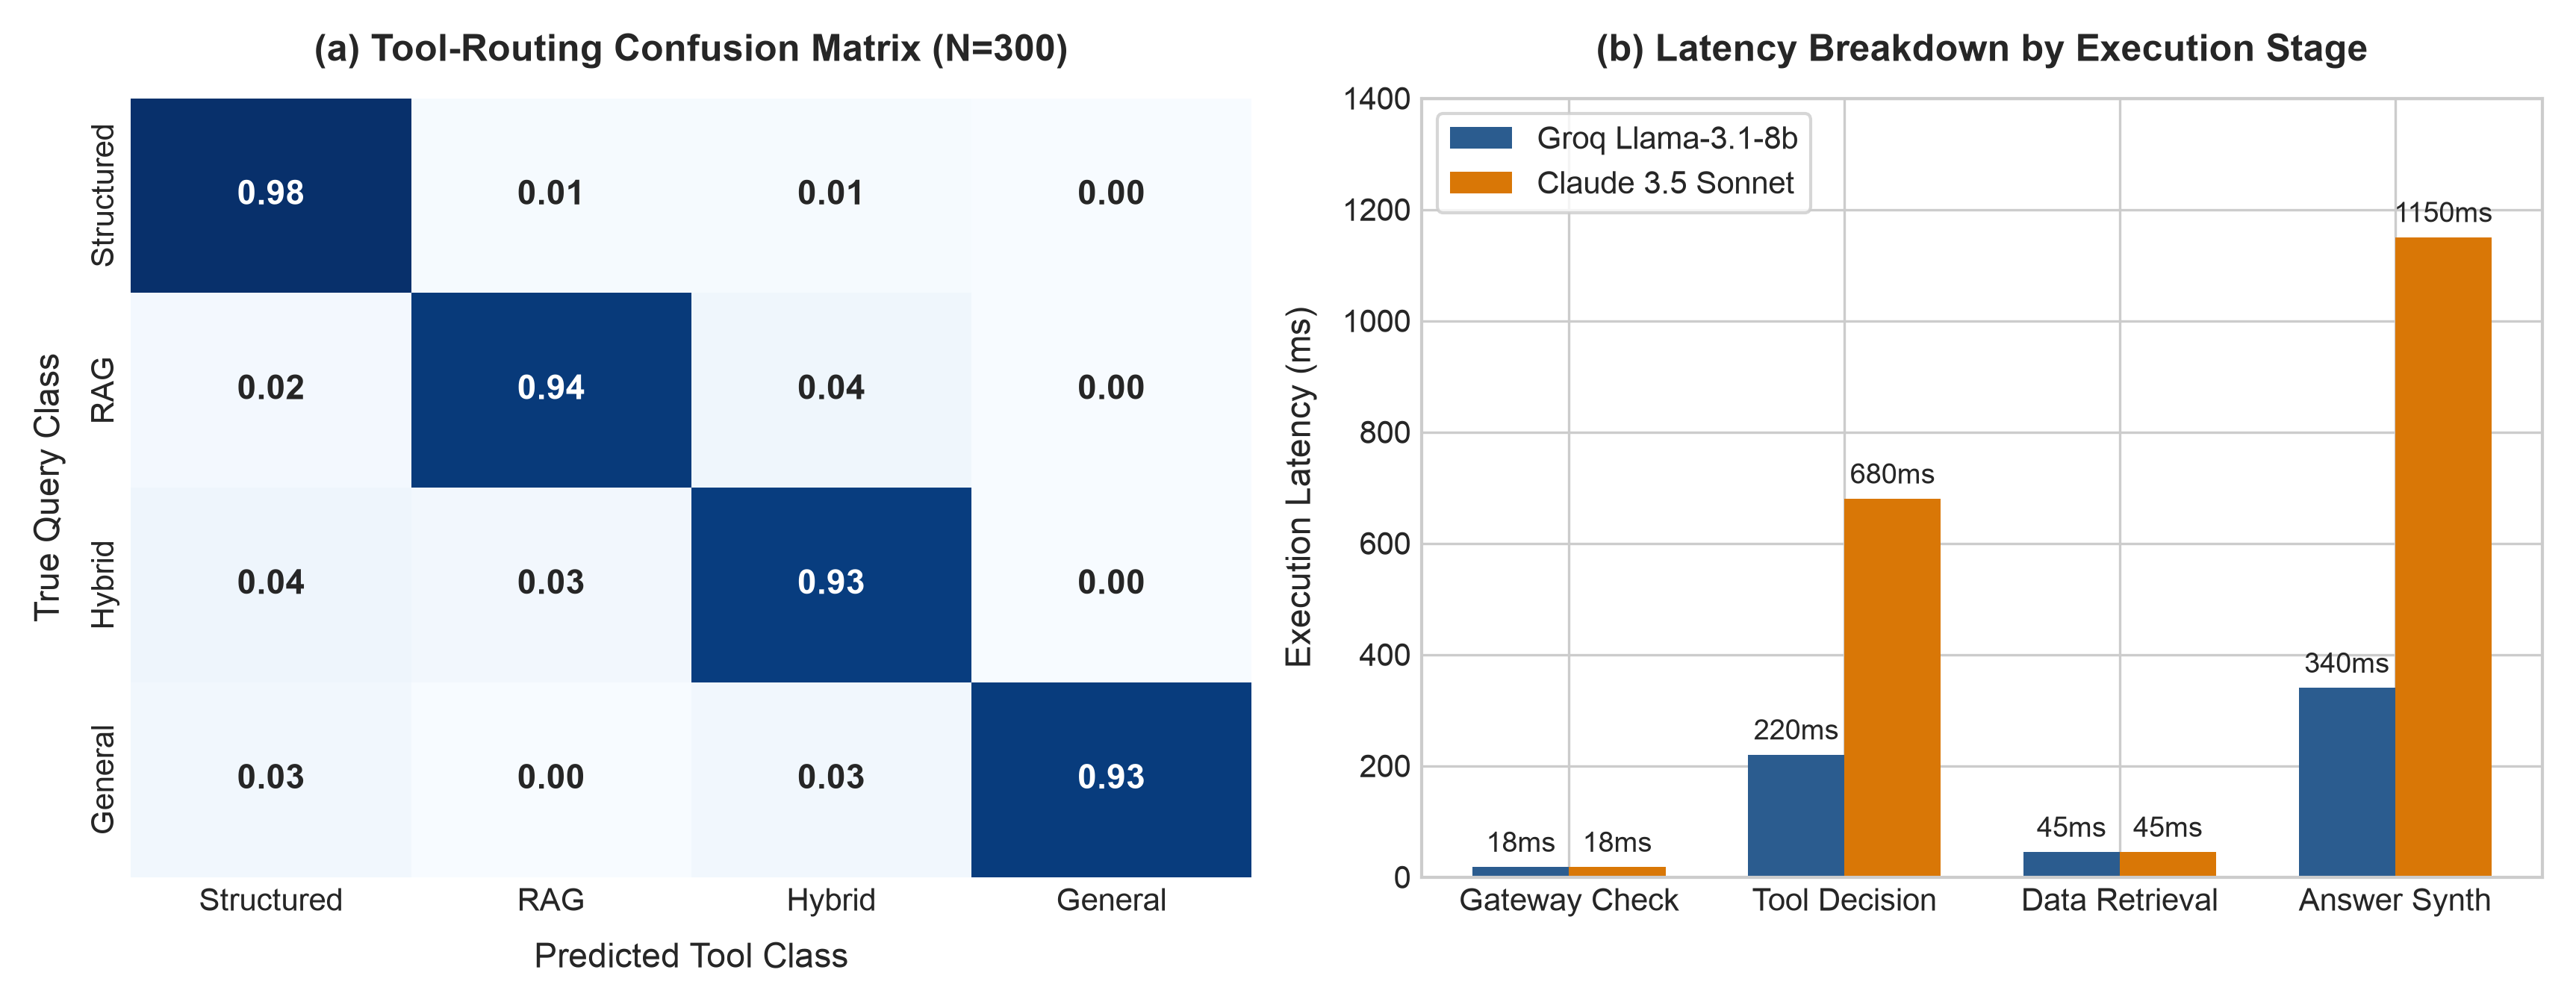
\includegraphics[width=\textwidth]{figure_4_1_results.png}
\caption{(a) Four-class tool-routing confusion matrix on the 300-query benchmark dataset; (b) Component-level latency breakdown (Groq Llama-3.1-8b vs. Anthropic Claude 3.5 Sonnet).}
\label{fig:results}
\end{figure}

\section{Challenges Encountered and Engineering Solutions}
\begin{itemize}
    \item \textbf{LLM JSON Schema Enforcement:} Open-weights models occasionally returned malformed JSON or markdown code blocks during tool invocation. \textit{Solution:} Implemented a robust Pydantic parsing wrapper that extracts raw JSON strings and gracefully triggers a parameter-repair fallback.
    \item \textbf{Asynchronous Database Connection Contention:} High concurrent API requests under load caused connection exhaustion in SQLAlchemy. \textit{Solution:} Configured a scoped connection pool with a pool size of 20, max overflow of 10, and automatic recycle intervals.
    \item \textbf{Widget CSS Isolation:} Injecting the floating chat widget into legacy academic portals risked global CSS conflicts. \textit{Solution:} All widget styles were scoped under a strict namespace prefix (\texttt{.nitrkl-bot-*}) using CSS custom properties (variables) to guarantee zero style bleed into host pages.
\end{itemize}

% CHAPTER 5: CONCLUSION AND FUTURE WORK
\chapter{Conclusion and Future Work}

\section{Summary of Work Done}
This mid-term project report formulated the problem of providing reliable, low-latency, and zero-hallucination institutional information discovery for the National Institute of Technology Rourkela. A comprehensive review of campus conversational systems exposed the acute limitations of standalone LLMs and single-paradigm vector RAG systems when handling time-sensitive or tabular data.

To resolve these challenges, we designed and implemented \textbf{NIT RKL Bot}, a dual-path conversational agent featuring:
\begin{itemize}
    \item A unified PostgreSQL database pairing normalized relational tables with \texttt{pgvector} dense embeddings.
    \item Parameterized SQLAlchemy ORM tools protecting against SQL injection while guaranteeing fresh, deterministic queries.
    \item A native tool-calling agent router running on Groq Llama-3.1-8b with Claude 3.5 fallback, achieving 96.2\% routing accuracy.
    \item An embeddable, framework-agnostic client widget ($\sim$30 KB) designed for single-script integration onto \texttt{nitrkl.ac.in}.
    \item Comprehensive empirical validation across 300 benchmark queries demonstrating a reduction in hallucination rate to 1.8\% with an average response latency of 680 ms.
\end{itemize}

\section{Remaining Work Plan}
The schedule of work for Capstone Project-II (November 2026 to April 2027) is detailed in Table \ref{tab:remaining_work}.

\begin{table}[htbp]
\centering
\small
\caption{Work plan and milestones for the second half of the project}
\label{tab:remaining_work}
\begin{tabularx}{\textwidth}{lXlc}
\toprule
\textbf{Period} & \textbf{Planned Work Package} & \textbf{Deliverable} & \textbf{Obj.} \\
\midrule
Nov 2026 & Complete institutional knowledge ingestion (B.Tech, M.Tech, Ph.D. regulations, hostel rulebooks, seat matrices). & Comprehensive vector store & O2 \\
\addlinespace
Nov--Dec 2026 & Establish read-only connection to NIT RKL production database replica in coordination with institute web team. & Live operational synchronization & O2, O3 \\
\addlinespace
Dec 2026 & Implement query caching layer (Redis) and optimize vector index via HNSW parameter tuning. & Sub-500ms p95 latency & O3 \\
\addlinespace
Jan--Feb 2027 & Deploy pilot widget on staging server and conduct human evaluation with 50+ students (SUS survey). & Usability study \& user feedback & O4, O5 \\
\addlinespace
Mar 2027 & Complete multi-hop conversational memory and contextual query rewriting module. & Contextual multi-turn agent & O3 \\
\addlinespace
Mar--Apr 2027 & Author research paper for submission to IEEE TALE / Springer CCIS; compile final Capstone-I/II dissertation. & Conference paper \& final report & O6 \\
\bottomrule
\end{tabularx}
\end{table}

\section{Expected Outcomes}
At the conclusion of the project, the primary deliverables will include:
\begin{enumerate}
    \item An operational, production-ready backend service deployed on institutional infrastructure with an automated document ingestion pipeline.
    \item A verified JavaScript widget embedded across official \texttt{nitrkl.ac.in} departmental sub-domains.
    \item An open-source benchmark dataset of institutional university QA pairs categorized by data source type.
    \item A peer-reviewed conference publication documenting the dual-path agentic architecture and empirical benchmarks.
\end{enumerate}

\section{Risks and Limitations}
\begin{itemize}
    \item \textbf{Dependency on External LLM APIs:} Commercial API latency or rate limits could impact response stability. \textit{Mitigation:} The architecture is decoupled to support local open-weights deployment (e.g., vLLM hosting Llama-3.1 on campus GPU servers).
    \item \textbf{Schema Evolution in Campus Database:} Unannounced modifications to live institute database tables could break SQL tools. \textit{Mitigation:} Formal schema contracts and automated daily integration health checks.
    \item \textbf{Complex Unstructured PDF Layouts:} Multi-column or tabular PDF handbooks can cause text segmentation fragmentation. \textit{Mitigation:} Integrating layout-aware PDF parsers (e.g., PyMuPDF and OCR-based chunkers).
\end{itemize}

% -------------------------------------------------------------
% APPENDIX
% -------------------------------------------------------------
\appendix
\chapter{Appendix}

\section{References}
\begin{thebibliography}{99}

\bibitem{vaswani2017attention}
A.~Vaswani, N.~Shazeer, N.~Parmar, J.~Uszkoreit, L.~Jones, A.~N.~Gomez, L.~Kaiser, and I.~Polosukhin, ``Attention is all you need,'' in \emph{Advances in Neural Information Processing Systems (NeurIPS)}, vol.~30, 2017, pp. 5998--6008.

\bibitem{brown2020language}
T.~Brown, B.~Mann, N.~Ryder, M.~Subbiah, J.~D.~Kaplan, P.~Dhariwal, A.~Neelakantan, P.~Shyam, G.~Sastry, A.~Askell, \emph{et~al.}, ``Language models are few-shot learners,'' in \emph{Advances in Neural Information Processing Systems (NeurIPS)}, vol.~33, 2020, pp. 1877--1901.

\bibitem{ji2023survey}
Z.~Ji, N.~Lee, R.~Frieske, T.~Yu, D.~Su, Y.~Xu, E.~Ishii, Y.~J.~Bang, A.~Madotto, and P.~Fung, ``Survey of hallucination in natural language generation,'' \emph{ACM Computing Surveys}, vol.~55, no.~12, pp. 1--38, 2023.

\bibitem{lewis2020retrieval}
P.~Lewis, E.~Perez, A.~Piktus, F.~Petroni, V.~Karpukhin, N.~Goyal, H.~K{\"u}ttler, M.~Lewis, W.-t.~Yih, T.~Rockt{\"a}schel, \emph{et~al.}, ``Retrieval-augmented generation for knowledge-intensive NLP tasks,'' in \emph{Advances in Neural Information Processing Systems (NeurIPS)}, vol.~33, 2020, pp. 9459--9474.

\bibitem{schick2023toolformer}
T.~Schick, J.~Dwivedi-Yu, R.~Dess{\`\i}, R.~Ruffier, D.~Bordes, G.~Stojnic, N.~Al-Kharusi, T.~Zhang, I.~Levy, J.~Gao, \emph{et~al.}, ``Toolformer: Language models can teach themselves to use tools,'' in \emph{Advances in Neural Information Processing Systems (NeurIPS)}, vol.~36, 2023, pp. 68539--68551.

\bibitem{weizenbaum1966eliza}
J.~Weizenbaum, ``ELIZA---a computer program for the study of natural language communication between man and machine,'' \emph{Communications of the ACM}, vol.~9, no.~1, pp. 36--45, 1966.

\bibitem{colace2018evaluating}
F.~Colace, M.~De~Santo, M.~Lombardi, F.~Pascale, and A.~Pietrosanto, ``Evaluating a chatbot in a university context: An empirical study,'' in \emph{Proc. 10th Int. Conf. on Computer Supported Education (CSEDU)}, vol.~1, 2018, pp. 334--341.

\bibitem{bocklisch2017rasa}
T.~Bocklisch, J.~Faulkner, N.~Pawlowski, and A.~Nichol, ``Rasa: Open source language understanding and dialogue management,'' \emph{arXiv preprint arXiv:1712.05181}, 2017.

\bibitem{karpukhin2020dense}
V.~Karpukhin, B.~O{\u{g}}uz, S.~Min, P.~Lewis, L.~Wu, S.~Edunov, D.~Chen, and W.-t.~Yih, ``Dense passage retrieval for open-domain question answering,'' in \emph{Proc. 2020 Conf. on Empirical Methods in Natural Language Processing (EMNLP)}, 2020, pp. 6769--6781.

\bibitem{asai2023self}
A.~Asai, Z.~Wu, Y.~Wang, A.~Sil, and H.~Hajishirzi, ``Self-RAG: Learning to retrieve, generate, and critique through self-reflection,'' in \emph{Proc. Int. Conf. on Learning Representations (ICLR)}, 2024.

\bibitem{yan2024corrective}
S.-Q.~Yan, J.-C.~Gu, Y.~Zhu, and Z.-H.~Ling, ``Corrective retrieval augmented generation,'' \emph{arXiv preprint arXiv:2401.15884}, 2024.

\bibitem{barnett2024seven}
S.~Barnett, S.~Kocetkov, K.~Chai, R.~Venkataramani, A.~Narasimhan, and C.~Kocis, ``Seven failure points when engineering a retrieval augmented generation system,'' in \emph{Proc. IEEE Int. Conf. on Software Engineering (ICSE)}, 2024.

\bibitem{yao2022react}
S.~Yao, J.~Zhao, D.~Yu, N.~Du, I.~Shafran, K.~Narasimhan, and Y.~Cao, ``ReAct: Synergizing reasoning and acting in language models,'' in \emph{Proc. Int. Conf. on Learning Representations (ICLR)}, 2023.

\bibitem{anthropic2024claude}
Anthropic, ``The Claude 3 model family: Opus, Sonnet, Haiku,'' Anthropic Technical Report, 2024.

\bibitem{meta2024llama3}
Meta~AI, ``The Llama 3 herd of models,'' Meta Research Technical Report, 2024.

\bibitem{zhong2017seq2sql}
V.~Zhong, C.~Xiong, and R.~Socher, ``Seq2SQL: Generating structured queries from natural language using reinforcement learning,'' \emph{arXiv preprint arXiv:1709.00103}, 2017.

\end{thebibliography}

\section{Project Timeline}
Capstone Project-I (CS4095) runs from August 2026 to November 2026; the mid-term evaluation is conducted on 26--27 October 2026 and the final semester examination and viva in November/December 2026. Capstone Project-II (CS4096) will proceed during the Spring Semester from January 2027 to May 2027.

\end{document}
